\documentclass[11pt, spanish, a4paper, twoside]{article}

% Versión 1.er cuat 2021 Víctor Bettachini < vbettachini@unlam.edu.ar >

\usepackage[T1]{fontenc}
\usepackage[utf8]{inputenc}

\usepackage[spanish, es-tabla]{babel}
% \def\spanishoptions{argentina} % Was macht dass?
% \usepackage{babelbib}
% \selectbiblanguage{spanish}
% \addto\shorthandsspanish{\spanishdeactivate{~<>}}


\usepackage{graphicx}
\graphicspath{{./figuras/}{../LaTeX/}{../figurasLaTeX/}{./figs}}
% \usepackage{float}

\usepackage[arrowdel]{physics}
\newcommand{\pvec}[1]{\vec{#1}\mkern2mu\vphantom{#1}}
% \usepackage{units}
\usepackage[separate-uncertainty= true, multi-part-units= single, range-units= single, range-phrase= {~a~}, locale= FR]{siunitx}
\usepackage{isotope} % $\isotope[A][Z]{X}\to\isotope[A-4][Z-2]{Y}+\isotope[4][2]{\alpha}

\usepackage{tasks}
\usepackage[inline]{enumitem}
% \usepackage{enumerate}

\usepackage{hyperref}

% \usepackage{amsmath}
% \usepackage{amstext}
% \usepackage{amssymb}

\usepackage{tikz}
\usepackage{tikz-3dplot}
\usepackage{tikz-dimline}
\usetikzlibrary{calc}
% \usetikzlibrary{math}
\usetikzlibrary{arrows.meta}
\usetikzlibrary{snakes}
\usetikzlibrary{decorations}
\usetikzlibrary{decorations.pathmorphing}
\usetikzlibrary{patterns}

\usepackage[hmargin=1cm,vmargin=3cm, top= 0.75cm,nohead]{geometry}

\usepackage{lastpage}
\usepackage{fancyhdr}
\pagestyle{fancyplain}
\fancyhf{}
\setlength\headheight{28.7pt} 
\fancyhead[LE, LO]{\textbf{Mecánica Analítica Computacional} }
% \fancyhead[LE, LO]{\textbf{Mecánica General} }
\fancyhead[RE, RO]{\href{https://ingenieria.unlam.edu.ar/}{$\vcenter{\hbox{
\includegraphics[height=1cm]{ambos.pdf}}}$}}
\fancyfoot{\href{https://creativecommons.org/licenses/by-nc-sa/4.0/deed.es_ES}{$\vcenter{\hbox{
\includegraphics[height=0.4cm]{by-nc-sa_80x15.pdf}}}$} \href{https://ingenieria.unlam.edu.ar/}{DIIT - UNLaM}}
\fancyfoot[C]{ {\tiny Actualizado al \today} }
\fancyfoot[RO, LE]{Pág. \thepage/\pageref{LastPage}}
\renewcommand{\headrulewidth}{0pt}
\renewcommand{\footrulewidth}{0pt}

% LTeX: language = es-AR
% \usepackage{svg}

\begin{document}
\begin{center}
  % \textsc{\large Mecánica general}\\
  \textsc{\large Cuerpo rígido | Ecuaciones de Euler}
\end{center}

% De poder resolver estos problemas en forma autónoma puede asumir que adquirió los conocimientos mínimos sobre los temas abordados en la semana. No dude en consultar a docentes y compañeros si no puede terminarlos. Los problemas marcados con * son opcionales.

\begin{enumerate}

	\item 
	\begin{minipage}[t][5cm]{0.55\textwidth}
		\textbf{Engranaje inclinado}
		Un engranaje de masa de \SI{10}{\kilo\gram} está montado con una inclinación de \ang{10;;} en un eje de masa despreciable.
		Los cojinetes \(A\) y \(B\) sostienen el eje que gira con velocidad angular constante.
		El \(A\) es de empuje, por lo que provee reacción también en la dirección longitudinal al eje en tanto que el \(B\) solo lo hace en las direcciones transversales.
		Los momentos de inercia del engranaje son \(I_z = \SI{.1}{\kilo\gram\metre\squared}\) y el \(I_y = \SI{.05}{\kilo\gram\metre\squared}\).
		\begin{tasks} 
			\task Determine las reacciones que deben proveer los cojinetes para el instante en que el sistema en rotación presenta la disposición que se ilustra.
		\end{tasks}
	\end{minipage}
	\begin{minipage}[c][0.5cm][t]{0.4\textwidth}
		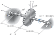
\includegraphics[width=\textwidth]{hibb_21-4}
		% 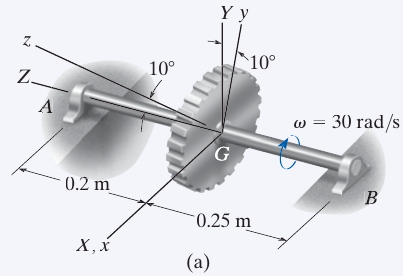
\includegraphics[width=\textwidth]{hibb21_4}
	\end{minipage}


	\item 
	\begin{minipage}[t][4.6cm]{0.55\textwidth}
		\textbf{Volante de inercia}
		El volante de inercia centrado en \(G\) tiene una masa de \SI{10}{\kilo\gram} es solidario al eje de masa despreciable que gira con velocidad angular constante \(\omega_s= \SI{6}{\per\second} \) (radianes por segundo) sostenido por los cojinetes \(A\) y \(B\).
		El primero es de empuje, por lo que provee reacción también en la dirección longitudinal al eje en tanto que el segundo solo lo hace en las direcciones transversales.
		Un eje transversal al del volante sostiene la montura del cojinete \(A\) y también gira con velocidad angular constante \(\omega_p\).
		\begin{tasks}
			\task Determine las reacciones que proveen los cojinetes.
		\end{tasks}
	\end{minipage}
	\begin{minipage}[c][0.5cm][t]{0.4\textwidth}
		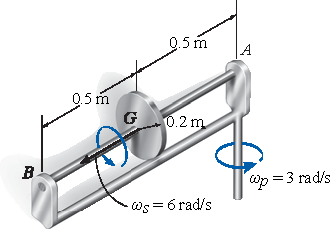
\includegraphics[width=\textwidth]{hibb_21-6}
		% \includesvg[width=\textwidth]{hibb_21-6.svg}
		% 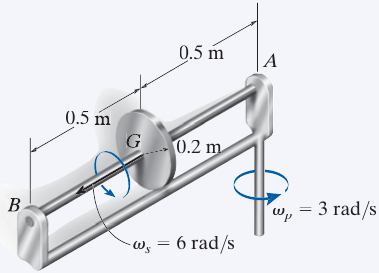
\includegraphics[width=\textwidth]{hibb21_6}
	\end{minipage}


	\item
	\begin{minipage}[t][3cm]{0.75\textwidth}
		\textbf{Rotación fuera de eje}
		Un cilindro homogéneo de masa \(m\), radio \(R\) y altura \(H\) gira con velocidad angular constante \(\vec{\omega}\) en torno a un eje que forma un ángulo de \ang{30;;} con el \(\hat{z}\) y que pasa por su centro de masa.
		\begin{tasks}
			\task Calcular el torque que debe aplicarse al cilindro para mantener tal movimiento.
		\end{tasks}
	\end{minipage}
	\begin{minipage}[c][2cm][t]{0.2\textwidth}
		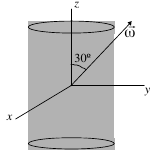
\includegraphics[width=\textwidth]{Ex3_17}
	\end{minipage}



	\item 
	\begin{minipage}[t][4.5cm]{0.75\textwidth}
		\textbf{Barra en rotación}
		La barra delgada AB tiene una masa \(m\) y está conectada al soporte por medio de un pasador en A.
		El soporte está rígidamente montado en la flecha.
		Determine la velocidad angular constante requerida \(\omega\) de la flecha, para que la barra forme un ángulo \(\theta\) con la vertical.
	\end{minipage}
	\begin{minipage}[c][3cm][t]{0.2\textwidth}
		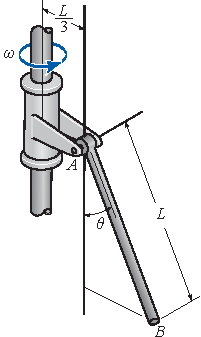
\includegraphics[width=\textwidth]{hibb_21-45}
	\end{minipage}


	\item 
	\begin{minipage}[t][3.5cm]{0.6\textwidth}
	\textbf{Cilindro desbalanceado}
		Un cilindro de altura \(D\) y masa \(M\) gira apoyado en dos cojinetes \(P\) y \(Q\) con velocidad angular \(\omega\).
		En un eje imaginario en un ángulo \(\varphi\) del eje de rotación, y a una distancia \(a\) de su centro, tiene colocadas dos pesas de igual masa, \(m\). 
		\begin{tasks} 
			\task Calcular la fuerza que aplican los cojinetes.
		\end{tasks}
	\end{minipage}
	\begin{minipage}[c][0.5cm][t]{0.35\textwidth}
		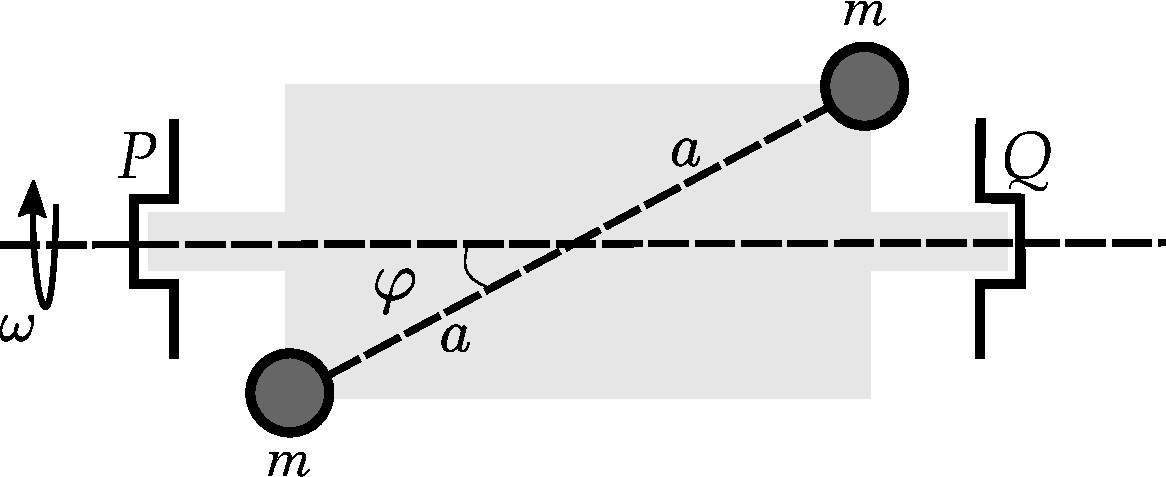
\includegraphics[width=\textwidth]{cilindroDesbalanceado}
	\end{minipage}
		

	\item 
	\begin{minipage}[t][4.5cm]{0.55\textwidth}
		\textbf{``Flecha'' sobre cojinetes}
		La flecha se construyó con una barra cuya masa por unidad de longitud es de \SI{2}{\kilo\gram\per\metre}.
		Determine las componentes \(x, y, z\) de la reacción en los cojinetes A y B si en el instante que se muestra la flecha gira libremente a una velocidad angular de \(\omega = \SI{30}{\per\second}\) (radianes por segundo).
		¿Cuál es la aceleración angular de la flecha en este instante?
		El cojinete A es capaz de soportar una componente de fuerza en la dirección y mientras que el cojinete B no.
		Ignore la masa del eje.
	\end{minipage}
	\begin{minipage}[c][0cm][t]{0.4\textwidth}
		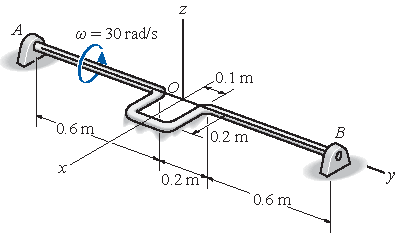
\includegraphics[width=\textwidth]{hibb_21-48}
	\end{minipage}


	\item 
	\begin{minipage}[t][6.5cm]{0.65\textwidth}
		\textbf{Aceleración angular constante}
		El cilindro de 15 libras rota alrededor del eje AB con \(\vec{\omega} = -\SI{4}{\per\second} \hat{x}\) (radianes por segundo).
	El cojinete \(A\) no soporta fuerza en el sentido de \(x\) de lo que se ocupa el \(B\).
	El eje que parte del soporte en su punto \(C\), que parte del reposo, está sometido a una aceleración \(\vec{\alpha}_C = \dot{\vec{\omega}} = \SI{12}{\per\second\squared} \hat{Z}\) (radianes por segundo cuadrado), siendo que \(\hat{Z}\) incluye a \(\overline{AC}\) y es paralelo a \(\hat{z}\).
	\begin{tasks}
		\task Convierta los datos en unidades imperiales (pies, libras) en unidades del Sistema Internacional.
		\task Determine las reacciones que deben proveer los cojinetes.
	\end{tasks}
	\end{minipage}
	\begin{minipage}[c][2cm][t]{0.3\textwidth}
		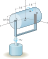
\includegraphics[width=\textwidth]{hibbEng_21-58}
		% 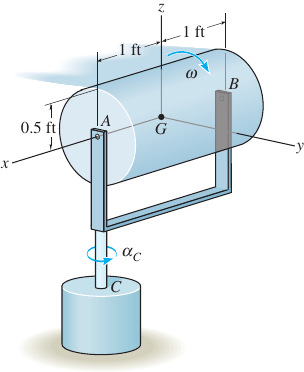
\includegraphics[width=\textwidth]{hibb_14_21_58}
	\end{minipage}


	\item 
	\begin{minipage}[t][3.5cm]{0.65\textwidth}
		\textbf{Trituradora de roca}
		Una trituradora de roca se compone de un disco delgado grande el cual está conectado por medio de un pasador a un eje horizontal.
		Si éste gira a una velocidad constante de \SI{8}{\per\second} (radianes por segundo), determine la fuerza normal que el disco ejerce en las piedras.
		Suponga que el disco rueda sin deslizarse y que su masa es de \SI{25}{\kilo\gram}.
		Ignore la masa del eje.
	\end{minipage}
	\begin{minipage}[c][2cm][t]{0.3\textwidth}
		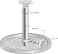
\includegraphics[width=\textwidth]{hibb_21-56}
	\end{minipage}


\end{enumerate}

\end{document}
